\begin{document}
	

\subsection{Exercise}\label{sec:exercise}
Consider the following program and the table \ref{chex1-table-dc} of energy consumption in the different states. Compute:
\begin{itemize}
	\item the energy consumption of the device per single hour
	\item the expected lifetime of the device
\end{itemize}
\begin{lstlisting}
	void loop(){
		
		//4 milliseconds
		turnOn(analogSensor);
		int sensorValue = analogRead(A0);
		turnOff(analogSensor);
		
		// 1 milliseconds
		float voltaage = sensorValue*(5.0/1023.0);
		
		//15 milliseconds
		turnOn(radioInterface);
		Serial.println(voltage);
		turnOff(radioInterface);
		
		//380 milliseconds
		idle(380);
		
	}
\end{lstlisting}

\begin{figure}[h]
	\centering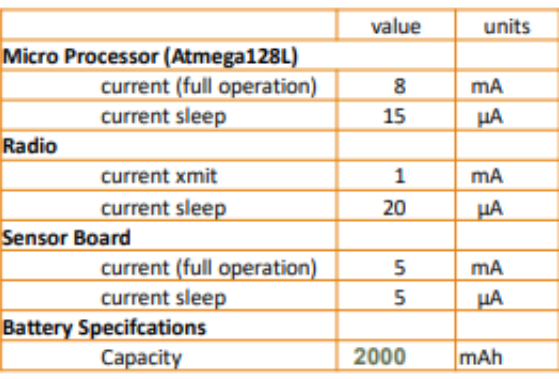
\includegraphics[scale=0.45]{images/Pasted image 20230508152346.png}
	\caption{Exercise 1 parameters}
	\label{chex1-table-dc}
\end{figure}



\subsubsection{Answer}\label{sec:answer}
Consider the energy consumption per hour:
\begin{enumerate}
	\item The processor has a duty cycle of:
	
	\item The radio has a duty cycle of:
	\item The sensor has a duty cycle of:
	\item The energy consumption in one hour is:
	\item The lifetime of the device is: 
\end{enumerate}



\subsubsection{Exercise 2}\label{sec:exercise-2}
Consider the sensor specification in the table pictured in \ref{chenergy-ex2}
\begin{figure}
	\centering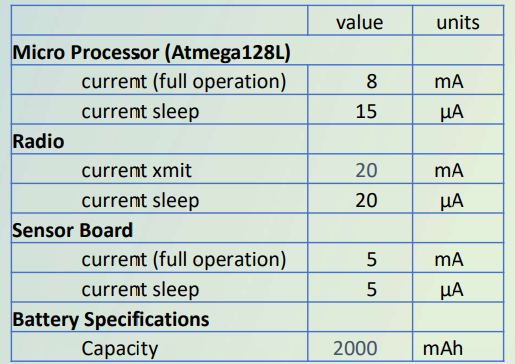
\includegraphics[scale=0.50]{images/Pasted image 20230328161140.png}
	\caption{Exercise 2 - Parameters specification}
	\label{chenergy-ex2}
\end{figure}


The device measures the hearth-rate (HR) of a person:
\begin{itemize}
	\item 
	Samples a photo-diode on the wrist at 20 Hz
	\begin{itemize}
		\item 
		sampling the sensor takes 0.5 ms
		\item 
		it requires both the processor and the sensor active
	\end{itemize}
	\item 
	HR is computed every 2 s (based on 40 samples)
	\item 
	Transmit (from time to time… see below) a data packet to the server:
	\begin{itemize}
		\item 
		The average time required to transit is 2 ms
		\item 
		Requires both processor and radio active
		Compute the energy consumption and the lifetime of the device if it sends all the samples to a server:
	\end{itemize}
	\item 
	Stores 5 consecutive samples from the photodiode
	\item 
	Transmits the stored 5 samples to the server
	\item 
	The server computes HR (hence the device does not compute HR)
	Disregard battery leaks.
\end{itemize}
\subsubsection{Solution 2}\label{sec:solution-2}
\textbf{Duty cycle of sampling}: DC of processor + sensors: 0.5 milliseconds (sampling time) / 0.05 seconds  = (sampling period)= 0.01\\

\textbf{Duty cycle of transmitting}: DC of radio + processor: 2 milliseconds (transmit time) / 0,25 seconds (transmission period) = 0.008
\begin{itemize}
	\item Sensor power consumption:
	$E_{\eta} = 5 mAh * 0,01+ 5 uAh *0,99 =0,05+0,005 mAh = 0,055 mAh$
	\item Processor power consumption:
	$E_{\rho}=0,018*8 mAh + 0,982*15 uAh =0,144+0,0147 mAh = 0,1587 mAh$
	\item Radio power compsution:
	$E_{\lambda}=0,008*20 mA + 0,99992*20\eta A = 0.16 mA + 0.0198 mA = 0.1799 mAh$
\end{itemize}

\begin{center}
	$E = E_{\eta} + E_{\rho} + E_{\lambda}$\\
	Battery specification (\textit{in table}) $B_{0} = 2000mAh$\\
	Power consumption: $2000 mAh / 0,3935 mAh$     $(\frac{B_{0}}{E})$\\
	obtaining \textbf{Lifetime}:  $5082 h$
\end{center}




\subsection{Exercise 3}
Consider the sensor specification in the table pictured in \ref{chenergy-ex3}.
\begin{figure}
	\centering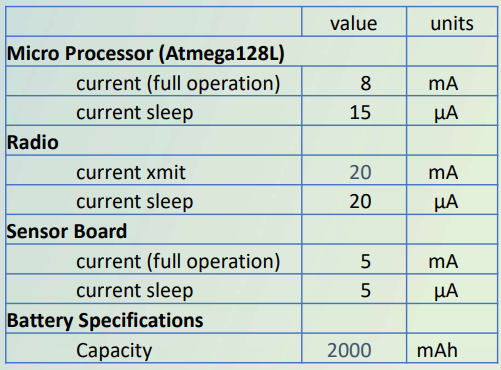
\includegraphics[scale=0.50]{images/Pasted image 20230328162514.png}
	\caption{Exercise 3 - Parameters specification}
	\label{chenergy-ex3}
\end{figure}

The device measures the hearth-rate (HR) of a person:
\begin{itemize}
	\item 
	Samples a photodiode on the wrist at 20 Hz
	\begin{itemize}
		\item 
		sampling the sensor takes 0.5 ms
		\item 
		it requires both the processor and the sensor active
	\end{itemize}
	\item 
	HR is computed every 2 s (based on 40 samples)
	\begin{itemize}
		\item 
		Computing HR in the device takes 5 ms
	\end{itemize}
	\item 
	Transmit a data packet to the server:
	\begin{itemize}
		\item 
		The average time required to transmit is 2 ms
		\item 
		Requires both processor and radio active
		Compute the energy consumption and the lifetime of the device if it computes HR itself:
	\end{itemize}
	\item 
	Transmits every 5 values of HR computed (1 packet every 10 seconds)
	
\end{itemize}
Disregard battery leaks.
\subsubsection{Solution 3}

\begin{itemize}
	\item Duty cycle of sampling: $0,5ms$ (sampling time) / $0,05s$ (sampling period)= $0,01$
	\item 
	Duty cycle of processing: 5 milliseconds / 2 seconds = 0,0025 
	\item 
	Duty cycle of transmitting: 2 milliseconds (transmit time) / 10 seconds (transmission period) = 0,0002
	\item 
	Power consumption of sensor (in 1h):
	\begin{itemize}
		\item 
		$E_{\eta} = 5 mAh * 0,01+ 5 uAh *0,99 =0,05+0,005 mAh = 0,055 mAh$
	\end{itemize}
	\item 
	Power consumption of processor (1h):
	\begin{itemize}
		\item 
		$E_{\rho} = 8 mAh * 0,0127+ 15 uAh *0,9873 =0,1016+0,0148 mAh = 0,1164 mAh$
	\end{itemize}
	\item 
	Power consumtpion of radio (1h):
	\begin{itemize}
		\item 
		$E_{\theta} = 0,0002 *20mAh + 0,9998 *20uAh = 0,004 + 0,02 mAh = 0,024 mAh$
		
		
	\end{itemize}
	
	\begin{center}
		$E = E_{\eta} + E_{\rho} + E_{\theta}$ = $0.1954 mAh$\\
		Battery specification (\textit{in table}) $B_{0} = 2000mAh$\\
		Power consumption: $2000 mAh / 0,1954 mAh$     $(\frac{B_{0}}{E})$\\
		Lifetime: $2000 mAh / 0,1954 mAh = 10.235 h$
	\end{center}
	
\end{itemize}


\subsection{Exercise 4}

Consider a Mote-class sensor with the parameters pictured in table \ref{chenergy-ex4}.
\begin{figure}
	\centering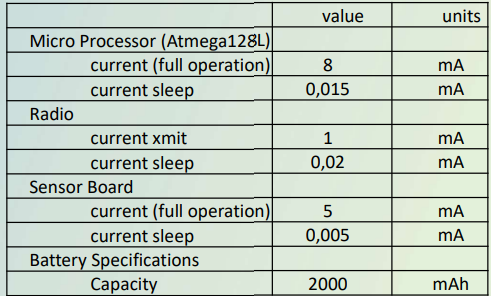
\includegraphics[scale=0.50]{images/Pasted image 20230328174646.png}
	\caption{Exercise 4 - Parameters specification}
	\label{chenergy-ex4}
\end{figure}


Assume that the device performs a sensing task with the following parameters:
\begin{itemize}
	\item 
	The sensor board is activated with a rate of 0,1 Hz to perform the sampling; this operation takes 0.5 milliseconds. At the end the sensor board is put in sleep mode. During each sensing operation the processor is always active.
	\item 
	After each sampling the processor performs a computation that takes 2 milliseconds.
	\item 
	Then the processor activates the radio and transmits the data. The transmission takes 1 millisecond and, during it, the processor is active. At the end the radio and the processor are both set in sleep mode.
	Compute the duty cycle of each component (\textit{sensor board, radio and processor}), and the lifetime of the device (\textit{assuming that the sensor stops working when its battery charge becomes 0}).
\end{itemize}
\paragraph{Solution 4}\label{sec:solution-4}\begin{itemize}
	\item 
	Sampling takes $0.5 ms$ with a rate of $0,1 Hz$
	\item 
	Processing: $2 ms$
	\item 
	Transmitting: 1 ms
	\item 
	\textbf{Duty cycle of sampling (processor and sensors)}: $0.5 ms /10s = 0,00005$
	\item 
	\textbf{Duty cycle of processing (only processor)}: $2ms/10s$  $(10000ms) = 0.0002$
	\item 
	\textbf{Duty cycle of transmissions (radio\&processor)}: $1ms/10s  = 0.0001$
	\item 
	Power consumption of sensor (in 1h):
	\begin{itemize}
		\item 
		$E_{\eta} = 5 mA * 0,00005+ 0,005 mA * (1-0,00005) = 2.5*10^{-4} mA + 0.05 mA = 0.00525 mA$
	\end{itemize}
	\item 
	Power consumption of processor (1h):
	\begin{itemize}
		\item 
		$E_{\rho} = 8 mA * 0.00035 + 0,015 mA *(1-0.00035) = 0.0028 mA+0,015 mA = 0,0178 mAh$
	\end{itemize}
	\item 
	Power consumtpion of radio (1h):
	\begin{itemize}
		\item 
		$E_{\theta} = 0,0001 * 1mA + (1-0,0001) *0,02 mA = 100 nA + 20 \eta A = 0.0201 mA$
		
	\end{itemize}
	\item \begin{center}
		$E = E_{\eta} + E_{\rho} + E_{\theta}$ = $0.04315 mAh$\\
		Battery specification (\textit{in table}) $B_{0} = 2000mAh$\\
		Power consumption: $2000 mAh / 0.04315 mAh$     $(\frac{B_{0}}{E})$\\
	\end{center}
	\textbf{Lifetime}: $2000 mAh / 0,04315 mAh = 46.349 h$
\end{itemize}


\subsection{Exercise 5}\label{sec:exercise}
Consider the following fragment of Arduino code:
% C null
\begin{lstlisting}
	void loop() { 
		int sensorValue = analogRead(A0);
		Serial.println(sensorValue); 
		delay(100);
	}
\end{lstlisting}

Compute its duty cycle assuming that:
\begin{itemize}
	\item 
	Reading an analog value takes 2 milliseconds
	\item 
	Transmitting along the serial line takes 5 milliseconds
\end{itemize}

\subsection{Exercise 6}\label{sec:exercise}
Consider an \textit{harvest-store-use} device with a \textbf{non-ideal energy buffer}:
\begin{itemize}
	\item 
	In the interval $[0, 10sec]$ the energy production is constant and produces $P_{s}(t) = 80 mA$
	\item 
	In the interval $[0, 4sec]$ the load is $P_{c}(t) = 150 mA$
	\item 
	In the interval $[4sec, 10sec]$ the load is $P_{c}(t) = 20 mA$
	\item 
	The charging efficiency is $\eta = 95\%$
	\item 
	The battery charge at time $0$ is $400 mAh$
	\item 
	The energy leak of the battery is negligible
	
\end{itemize}
Compute the battery charge at times $4sec$ and $10sec$.


\subsection{Exercise 7}\label{sec:exercise}
Consider a device that samples the battery output voltage with an analog to digital converter (ADC) at $10$ bits.
The battery has a maximum charge of $2000 mAh$, and its maximum voltage (\textit{when fully charged}) is $10$ Volts.
When the battery reaches a voltage of $8$ Volts the battery charge is $200mAh$ and it becomes insufficient to power the device.\\
Compute the \textbf{battery charge $B$} when the ADC outputs $920, 830, 1023$.
\paragraph{Solution}\label{sec:solution}
Summarize the data we already known:
\begin{itemize}
	\item 
	$d: 10$ bits
	\item 
	$B_{min}: 200mAh$
	\item 
	$B_{max}: 2000mAh$
	\item 
	$v_{min}: 8V$
	\item 
	$v_{max}: 10V$
\end{itemize}
Now compute:
\begin{itemize}
	\item 
	$x_{max} = 2^{d}-1 = 1023$
	\item 
	$x_{min} = ROUND [\frac{v_{min}}{v_{max}}\times (2^{d}-1)]=818$
\end{itemize}
Hence, when the ADC outputs:
\begin{itemize}
	\item 
	$x =920 \rightarrow B = 1096 mAh$ (\textit{half the charge})
	\item 
	$x = 830  \rightarrow B = 305 mAh$
	\item 
	$x = 1023  \rightarrow B = 2000mAh$ (\textit{full charge})
	
\end{itemize}
Remembering that $B = B_{min}+\frac{B_{max}-B_{min}}{x_{max}-x_{min}} \times (x-x_{min})$.


\subsection{Exercise 8}
The following table reports, for each slot in a day, the expected
energy production of an energy-harvesting IoT device.
Assuming that:
\begin{itemize}
	\item $dc_{max} = 90\%; p_{max} = 5mA; u(dc_{max}) = 100$
	\item $dc_{min} = 50\%; p_{min} = 1mA; u(dc_{min}) = 10$
\end{itemize}

Complete the table \ref{e7-table} by assigning a duty cycle, an utility, and a power
consumption to each slot, according to the Kansal’s algorithm.

\begin{figure}[h]
	\centering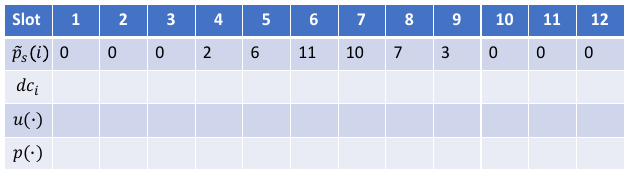
\includegraphics[scale=0.50]{images/Pasted image 20230601095844.png}
	\caption{Exercise 8 table}
	\label{e7-table}
\end{figure}


\subsection{Exercise 9}
In the Zigbee network in the figure \ref{e8-network}, built using
parameters $Rm=2, Dm=2 and Lm=3$, where purple
shaded nodes are routers and white nodes are end
devices, what range of addresses are assigned to
new router that joins the network in the following
cases:

\begin{itemize}
	\item  The new router joins as a child of router 1
	\item The new router joins as a child of router 20
	\item  The new router joins at node 7
\end{itemize}

\begin{figure}[h]
	\centering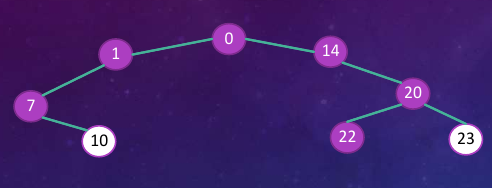
\includegraphics[scale=0.50]{images/Pasted image 20230601100433.png}
	\caption{Exercise 9 Network}
	\label{e8-network}
\end{figure}







\subsection{Questions 1}
Given the network in the figure \ref{wn-q1}, assume that the MAC protocol uses the RTS/CTS mechanism for the channel access.\\
Discuss which nodes detect themselves as hidden or exposed as
consequence of the RTS/CTS handshake in the following cases:
\begin{figure}[h!]
	\centering
	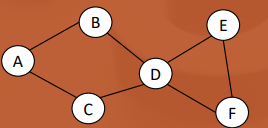
\includegraphics[scale=0.50]{images/Pasted image 20230531110613.png}
	\caption{Question 1 network schema}
	\label{wn-q1}
\end{figure}
\begin{itemize}
	\item Hidden terminals with respect to a transmission from E to D
	\item Hidden terminals with respect to a transmission from D to C
	\item Exposed terminals with respect to a transmission from D to B
	\item Exposed terminals with respect to a transmission from B to A
\end{itemize}



\subsection{Questions 2}\label{sec:questions-2}
Given the network in the previous figure \ref{wn-q1}:
\begin{itemize}
	\item assume that D hears the RTS sent by E but it does not hear the
	corresponding CTS. What does D can do?
	\item assume that B hears the CTS sent by D but it does not hear the
	corresponding RTS. What does B can do?
	\item Assume D is receiving a communication from a node, and B
	did not receive the corresponding RTS \& CTS and it does not
	hear the signal transmitted to D. If B wishes to transmit to D
	what happens?
\end{itemize}
The solution are:
\begin{itemize}
	\item 
	Exposed
	\item 
	Hidden
	\item 
	Collision
\end{itemize}


\subsection{Question 3}

\begin{figure}[h]
	\centering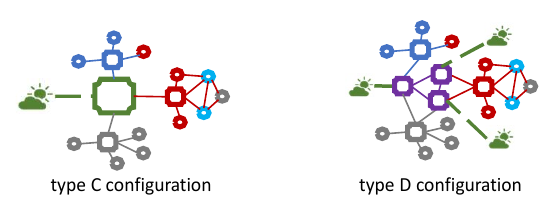
\includegraphics[scale=0.50]{images/Pasted image 20230601094121.png}
	\caption{Question 3 schema}
	\label{q3-schema}
\end{figure}

\begin{itemize}
	\item In type C configuration \ref{q3-schema}, how many mappings from one
	protocol to another (at the same level) the integration
	gateway should be able to manage?
	\item What about in type D configuration?
\end{itemize}


\subsection{Question 4}
Explain the meaning of the following topics used in a MQTT-based
system:
\begin{itemize}
	\item Pisa/neighborhood\_Cisanello/lamppost/TrafficSensor
	\item Pisa/neighborhood\_Cisanello/+/TrafficSensor
	\item Pisa/+/lamppost/\#
	\item Pisa/neighborhood\_Cisanello/\#
	\item \$SYS/broker/clients/total
\end{itemize}


\subsection{Question 5}
Consider the binding table and the address maps shown below \ref{q5-schema} that represent the state of the ZigBee network at time $t$. Assume device 0X0022 disconnects from the network at time $t'>t$ and it reconnects again at time $t''>t'$, obtaining network address 0X0003. Discuss to what network address and endpoint are delivered the following messages:

\begin{figure}[h]
	\centering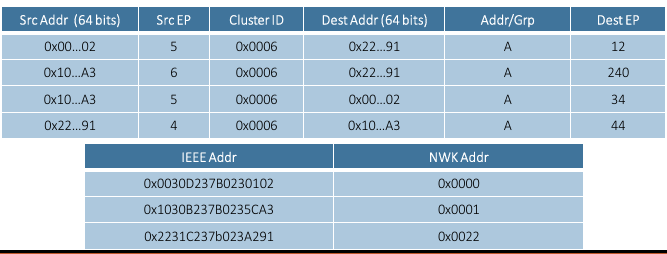
\includegraphics[scale=0.50]{images/Pasted image 20230601094724.png}
	\caption{Question 5 table}
	\label{q5-schema}
\end{figure}


\begin{itemize}
	\item Time $h<t'$ : message of cluster 0X0006 generated by device 0X0001 from endpoint 5
	\item 
	Time $h \in [t', t'']$: message of cluster 0X0006 generated by device 0X0000 from endpoint 5
	\item
	Time $h>t''$ : message of cluster 0X0006 generated by device 0X0022 from endpoint 4
	\item
	Time $h>t''$ : message of cluster 0X0006 generated by device 0X0001 from endpoint 6
\end{itemize}

\subsection{Question 6}
The radio of a device using BMAC takes 4.0 E-04 seconds to check for the preamble. Assuming that the frequency of the preamble sampling is 5/sec (that is, preamble sampling is performed 5 times in a second). What is the duty cycle of the preamble sampling activity?

\subsection{Question 7}
Referring the chapter on Direct Diffusion \ref{sec:directed-diffusion}, answer the following questions:
\begin{itemize}
	\item What is a gradient?
	\item Why does an interest is repeated  periodically? Isn’t the first one sufficient?
	\item How does the mechanism of directed diffusion may be used to
	optimize the underlying MAC layer?? (cross-layer optimization)
	\item In GPSR \ref{sec:greedy-perimeter-stateless-routing-gpsr}, when does a packet can switch back from
	perimeter mode to greedy mode?
\end{itemize}


\end{document}
